\apendice{Documentación de usuario}
\section{Requisitos software y hardware para ejecutar el proyecto.} \label{sec:requisitos}
A diferencia del entorno de desarrollo, el entorno de producción para el usuario final (el facultativo médico) se ha diseñado bajo la filosofía de \textit{Zero-Configuration} (Cero Configuración). El objetivo es que la curva de adopción técnica sea nula, evitando que el personal sanitario deba instalar librerías, configurar servidores locales o modificar variables de entorno. 

Para garantizar el correcto funcionamiento y despliegue del terminal clínico, el usuario o la institución hospitalaria únicamente deben asegurar el cumplimiento de los siguientes requisitos mínimos:

\subsubsection{Requisitos de \textit{Software}}
\begin{itemize}
    \item \textbf{Sistema Operativo:} El sistema es multiplataforma, pero para la ejecución en los equipos de escritorio de la unidad se requiere un Sistema Operativo \textit{Windows 10} o \textit{Windows 11} (arquitectura de 64 \textit{bits}). En el caso del uso del terminal portátil dedicado, este opera nativamente bajo \textit{Raspberry Pi OS} (basado en \textit{Debian}).
    \item \textbf{Navegador Web:} Al tratarse de una arquitectura basada en tecnologías web (\textit{framework Reflex}), la interfaz gráfica de usuario (\textit{UI}) se renderiza en el navegador. Se requiere una versión actualizada de navegadores modernos basados en \textit{Chromium} (\textit{Google Chrome}, \textit{Microsoft Edge}), \textit{Mozilla Firefox} o \textit{Apple Safari}.
    \item \textbf{Despliegue Centralizado y Acceso Inmediato:} No se requiere la instalación de \textit{Python}, dependencias externas ni \textit{software} local por parte de los facultativos de la \textit{URCCPQ}. La infraestructura de la aplicación y la base de datos se ejecutan de forma centralizada y transparente mediante contenedores \textit{Docker} en la \textit{intranet} del hospital. En consecuencia, el usuario interactúa con el sistema directamente a través de cualquier navegador web estándar, garantizando una adopción ágil y eliminando por completo la necesidad de mantenimiento o configuración en los equipos de la unidad.
\end{itemize}

\subsubsection{Requisitos de \textit{Hardware}}
El sistema no requiere de capacidades de procesamiento avanzadas (como tarjetas gráficas dedicadas), dado que el motor matemático optimizado exige un bajo consumo de recursos. Los requisitos físicos se dividen según la modalidad de uso:

\begin{itemize}
    \item \textbf{Uso en Equipos de Planta (\textit{Desktop}):} Cualquier ordenador estándar con un procesador de 64 \textit{bits}, un mínimo de 4\textit{GB} de memoria \textit{RAM}, conexión para periféricos de entrada (ratón y teclado) y espacio en disco suficiente para el almacenamiento de los archivos descargables.
    \item \textbf{Uso en el Terminal Portátil Dedicado:} Si se utiliza el dispositivo físico desarrollado en este proyecto, el \textit{hardware} ya se encuentra encapsulado y preconfigurado. El módulo consta de una placa \textit{Raspberry Pi 3 Model B}, una pantalla oficial \textit{LCD} táctil de 7 pulgadas y una tarjeta \textit{MicroSD} de 32\textit{GB}. El único requisito por parte del usuario es disponer de una fuente de alimentación estándar \textit{Micro-USB} conectada a la red eléctrica para recargar la batería.
\end{itemize}

\section{Puesta en marcha}
Esta sección proporciona una guía detallada para el despliegue y la primera puesta en funcionamiento del sistema. A diferencia de los métodos de instalación tradicionales que requieren la configuración manual de servidores, motores de bases de datos y entornos de ejecución, este proyecto implementa un modelo de \textbf{despliegue automatizado mediante contenedores \textit{Docker} en la \textit{intranet} del \textit{HUBU}}. 

Este enfoque garantiza que el facultativo pueda iniciar la plataforma de forma inmediata y segura, minimizando el riesgo de errores de configuración técnica.

\subsubsection{Acceso al Software desde los Equipos de Planta}
Gracias a la nueva arquitectura centralizada basada en contenedores \textit{Docker}, la plataforma opera como un servicio \textit{web} interno (\textit{On-Premise}\footnote{ Modelo de infraestructura donde el software y los servidores se instalan y operan dentro de las instalaciones físicas de la propia empresa, en lugar de en la nube.}). Por consiguiente, se elimina por completo la necesidad de instalar dependencias, descargar librerías o ejecutar \textit{scripts} locales en los ordenadores de la \textit{URCCPQ}. El procedimiento de acceso para cualquier facultativo se ha simplificado a los siguientes pasos:

\begin{enumerate}
    \item \textbf{Verificación de red:} Comprobar que el ordenador del puesto de trabajo está conectado a la \textit{intranet} del hospital. Este es un requisito técnico y legal indispensable, ya que el servidor opera en una red aislada sin salida a internet para garantizar la privacidad de los datos.
    
    \item \textbf{Acceso al portal:} Abrir el navegador \textit{web} institucional e introducir en la barra de direcciones la \textit{IP} local asignada al servidor (por ejemplo, \texttt{http://192.168.X.X:3000}) o su dominio interno correspondiente (ver Figura \ref{fig:acceso_navegador}).
    
    \begin{figure}[hbt!]
    		\centering
    		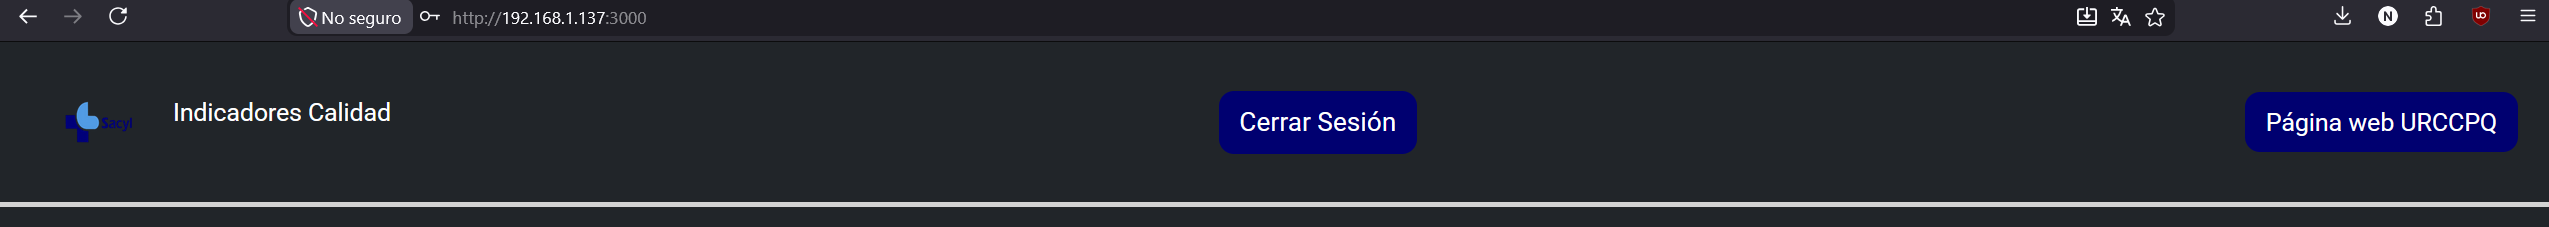
\includegraphics[width=1\textwidth]{img/ip.png}
    		\caption{Acceso a la plataforma clínica mediante la introducción de la \textit{IP} local en el navegador.}
    		\label{fig:acceso_navegador}
	\end{figure} 
	
    
    \item \textbf{Autenticación de usuario:} Una vez cargada la pantalla de inicio, el facultativo deberá introducir sus credenciales seguras. El sistema evaluará automáticamente su nivel de privilegios (\textit{RBAC}) y desplegará las herramientas y menús correspondientes a su rol operativo.
\end{enumerate}

A diferencia de las versiones previas de desarrollo, no existen ventanas de terminal (\textit{CMD}) ni procesos en segundo plano que el usuario deba gestionar, minimizar o monitorizar. Al finalizar la sesión clínica o la ingesta de datos, el usuario únicamente debe cerrar la pestaña del navegador para desvincularse de la aplicación de manera segura, sin riesgo de detener el servidor para el resto de la unidad. Para garantizar esta accesibilidad y transparencia de cara al facultativo, toda la complejidad de la plataforma se delega a la infraestructura del servidor. El entorno operativo se fundamenta en una orquestación de contenedores independientes que encapsulan la interfaz, el motor estadístico y la base de datos relacional de forma aislada. Como se puede observar en la Figura \ref{fig:docker_estado}, el motor de \textit{Docker} gestiona de forma centralizada el ciclo de vida de estos servicios, asegurando su ejecución ininterrumpida (\textit{Up}) y replicando con exactitud el comportamiento real que el sistema tendría al ser desplegado en los servidores de la \textit{intranet} hospitalaria.

	\begin{figure}[hbt!]
    		\centering
    		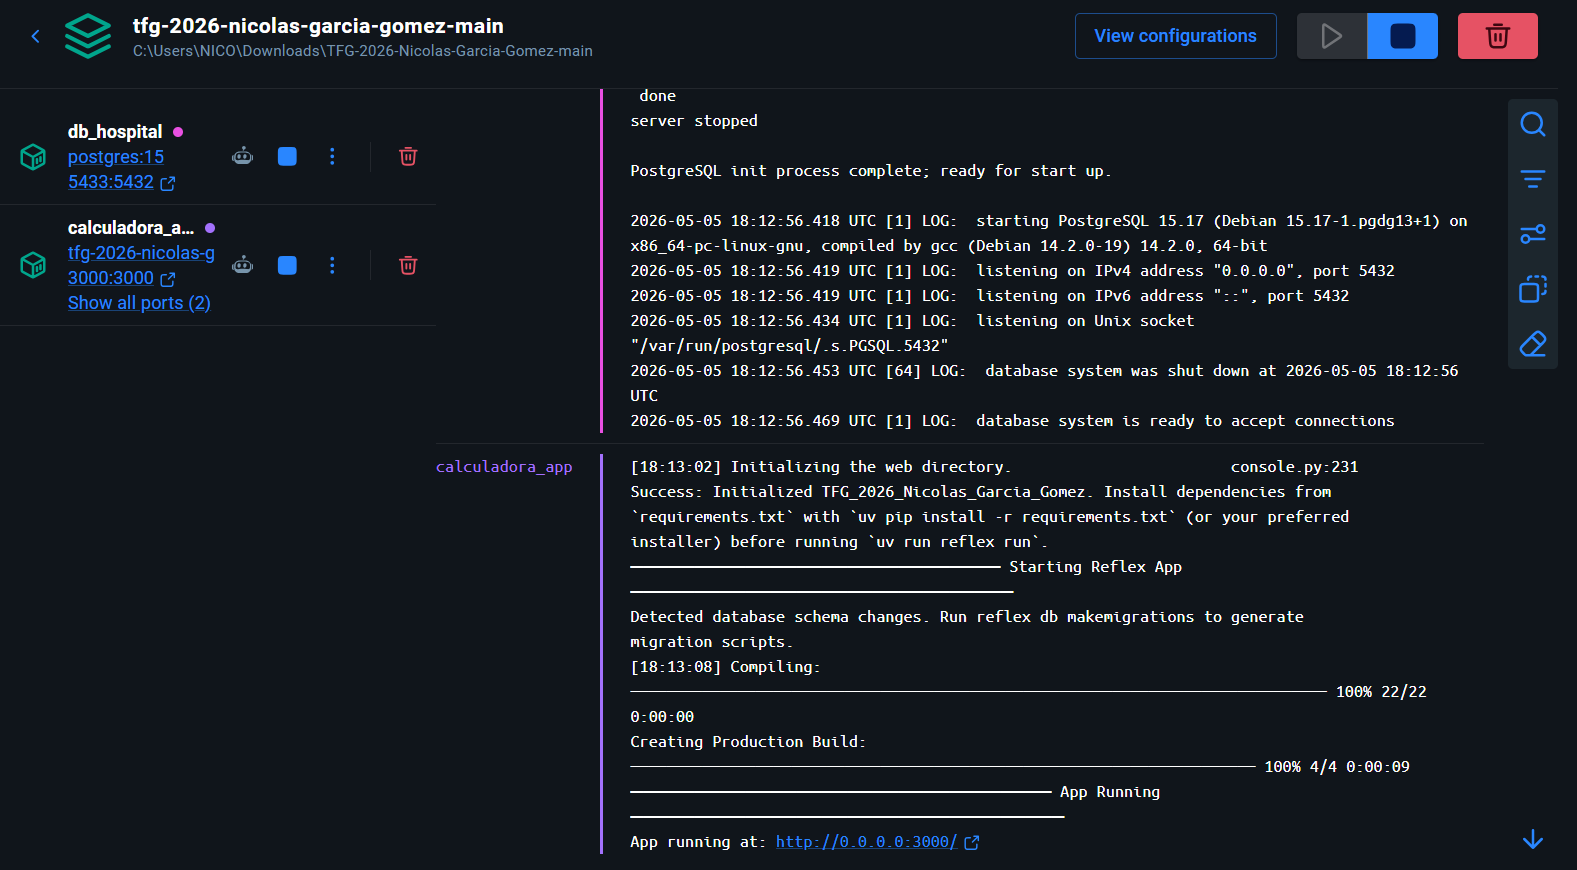
\includegraphics[width=0.85\textwidth]{img/consola_docker.png}
    		\caption{Panel de \textit{Docker} monitorizando el estado activo (\textit{Up}) de los contenedores que dan soporte a la plataforma en la \textit{intranet} simulada.}
    		\label{fig:docker_estado}
	\end{figure} 


\subsection{Guía de Operación del Terminal Físico}
Dado que el \textit{software} ha sido diseñado bajo una arquitectura de despliegue automatizado, la interacción del facultativo se centra principalmente en el manejo del dispositivo físico dedicado. A continuación, se detallan las pautas básicas para la correcta operación del terminal en la unidad de Reanimación (\textit{URCCPQ}).

\subsubsection{Encendido y Apagado}
El dispositivo cuenta con un sistema de gestión de energía integrado en su carcasa.
\begin{itemize}
    \item \textbf{Para encender el terminal:} Accione el interruptor físico situado en el lateral de la carcasa. La pantalla táctil se iluminará y el sistema operativo iniciará la plataforma clínica de forma automática en pocos segundos, mostrándose la pantalla de inicio lista para la carga de datos como se observa en la figura \ref{fig:terminal_fisico}.
    
    \begin{figure}[hbt!]
    		\centering
    		
\includegraphics[width=0.7\textwidth]{img/CabeceraEPS.png}
    		\caption{Terminal portátil encendido mostrando la interfaz inicial tras el arranque automático.}
    		\label{fig:terminal_fisico}
	\end{figure}

    \item \textbf{Para apagar el terminal:} Con el fin de evitar la corrupción de la tarjeta de memoria interna, se recomienda pulsar primero el botón de ``Apagar Sistema'' situado en el menú de la interfaz gráfica. Una vez la pantalla se apague por completo, puede accionar el interruptor lateral para cortar el suministro eléctrico de la batería.
\end{itemize}

\subsubsection{Autonomía y Recarga de la Batería}
El terminal está equipado con una batería interna de alta capacidad que le otorga total movilidad entre los distintos boxes de la unidad.
\begin{itemize}
    \item \textbf{Autonomía:} En condiciones de uso continuo y brillo de pantalla estándar, el dispositivo ofrece varias horas de autonomía operativa.
    \item \textbf{Proceso de carga:} Cuando el nivel de batería sea bajo, conecte un cable estándar con terminación \textit{Micro-USB} al puerto de carga habilitado en la carcasa, y conéctelo a un adaptador de red eléctrica de 5\textit{V}. 
    \item \textbf{Uso ininterrumpido:} Gracias a su módulo de gestión avanzada, el terminal puede seguir siendo utilizado con total normalidad mientras se encuentra enchufado recargando su batería, sin sufrir interrupciones ni reinicios.
\end{itemize}

\subsubsection{Cuidados y Limpieza}
Al tratarse de un dispositivo destinado a un entorno clínico de cuidados críticos, es importante mantener unas pautas de higiene que no comprometan la electrónica interna:
\begin{itemize}
    \item La carcasa, fabricada a medida mediante impresión \textit{3D}, protege los componentes internos. Sin embargo, el dispositivo \textbf{no es sumergible}.
    \item Para su desinfección superficial, se recomienda utilizar toallitas con alcohol isopropílico (al 70\textit{\%}) o paños de microfibra ligeramente humedecidos con soluciones desinfectantes de uso hospitalario, aplicándolos suavemente sobre la pantalla y la carcasa exterior.
    \item Evite la pulverización directa de líquidos sobre el terminal para prevenir filtraciones por las ranuras de ventilación o los puertos de conexión.
\end{itemize}

\section{Manuales y/o Demostraciones prácticas}
Para proceder a la utilización de la herramienta de calculo desarrollada, se requiere haber seguido las instrucciones de inicio automatizado descritas en el apartado anterior.

\subsubsection{Manual de Uso Clínico}
Este apartado resume las instrucciones necesarias para que cualquier facultativo pueda operar el sistema de forma autónoma, garantizando la integridad de los datos y la agilidad en la consulta.

\begin{enumerate}
    \item \textbf{Preparación del Entorno de Trabajo:} El procedimiento de inicialización dependerá del dispositivo utilizado para realizar el análisis clínico:
\begin{itemize}
    \item \textbf{Uso del Terminal Portátil (\textit{Raspberry Pi}):} Asegúrese de que el interruptor lateral del dispositivo esté en posición de encendido. Esto desplegará el servidor de forma local y autónoma, permitiendo el análisis de los archivos \textit{CSV} anonimizados extraídos previamente del hospital, sin necesidad de conexión a la red de la \textit{URCCPQ}.
    \item \textbf{Uso desde los Equipos de la Unidad:} Si se opera directamente desde los ordenadores de planta, no es necesaria la ejecución de ningún archivo o \textit{script} local. El sistema ya se encuentra desplegado de forma continua en la \textit{intranet}, por lo que bastará con acceder a la plataforma centralizada a través del navegador \textit{web}.
\end{itemize}
    \item \textbf{Navegación:} Una vez cargados los datos en la \textit{RAM}, utilice el menú lateral desplegable para alternar entre la vista de ``Resumen Indicadores'' (indicadores agregados de la unidad), la vista de ``Mezcla de Indicadores'' (permitiendo la comparación directa entre los indicadores) o seleccionando los indicadores individuales (profundización en una métrica específica).
    \item \textbf{Interacción con Gráficas:} Las gráficas permiten el filtrado dinámico. Al pasar el ratón sobre la leyenda de un indicador, este se mostrará en el lienzo principal, facilitando la limpieza visual durante la sesión.
\end{enumerate}

\subsubsection{Demostraciones prácticas}
Con el propósito de reducir el tiempo de aprendizaje del personal sanitario, se han realizado vídeos demostrativos accesibles desde los enlaces proporcionados:

\begin{itemize}
    \item \textbf{Vídeo ``\href{https://youtu.be/Yd4iXeUheLM}{Arranque de la Herramienta}'':} Vídeo del arranque normal del servidor.
    \item \textbf{Vídeo ``\href{https://youtu.be/rqjkfDiCUp4}{Uso Avanzado}'':} Tutorial sobre la carga de múltiples archivos \textit{.csv}, el uso de la \textit{BBDD} y de las diferentes funcionalidades de la \textit{web}.
    \item \textbf{Vídeo ``\href{https://www.overleaf.com}{Dispositivo Portátil}'':} Guía sobre el manejo físico, carga de batería y navegación básica por la interfaz táctil.
\end{itemize}



    
     